\documentclass[english, 11pt]{article}
\usepackage{../../notes}
\usepackage{lipsum}

%Global Course Variables
\newcommand{\myCourseCode}{EECS 442}
\newcommand{\myCourseName}{Computer Vision}
\newcommand{\myProf}{Matthew Johnson-Roberson}
\newcommand{\myTerm}{Fall 2015}
\newcommand{\myLogo}{../um_seal.png}

%Headers
\lhead{\myCourseName}
\rhead{\fancyplain{}{\rightmark}} 

%Footers
\cfoot{\thepage}

\begin{document}
\titleHeader{\myCourseCode}{\myCourseName}{\myProf}{\myTerm}{\myLogo}

%Document information
\rule[0.5ex]{1\columnwidth}{.5pt}
Contributors: Max Smith
\begin{center}
	Latest revision: \today
\end{center}
\toc
\abstr{Computational methods for the recovery, representation and application of visual information. Topics from image formation, binary images, digital geometry, similarity and dissimilarity detection, matching, curve and surface fitting, constraint propagation relaxation labeling, stereo, shading texture, object representation and recognition, dynamic scene analysis and knowledge based techniques. Hardware, software techniques.}

%----------------------------
%Document Begins
%----------------------------

\section{Introduction}
	\begin{itemize}
	\item See the syllabus.
\end{itemize}

\section{Linear Algebra \& Geometry}
	\subsection{Notation}
\begin{itemize}
	\item $x\in\mathbb{R}^D$: data 
	\item $\phi (x)\in\mathbb{R}^M$: features for $\vec{x}$
	\item $t\in\mathbb{R}$: continuous-valued labels
	\item $\vec{x}^{(n)}\equiv \vec{x}_n$: n-th training example
	\item $\vec{t}^{(n)}\equiv \vec{t}_n$: n-th targe value
\end{itemize}

\subsection{1D Inputs}
\begin{itemize}
	\item In the 1D case ($x\in\mathbb{R}^1$)
	\item Given a set of observations $x^{(1)},\ldots ,x^{(N)}$ and corresponding targe values $t^{(1)},\ldots,t^{(N)}$
	\item We want to learn a function $y(\vec{x}, W)\approx t$ to predict future values
	$$y(\vec{x}, \vec{w})=\sum_{j=0}^{M-1}\vec{w}_j \phi_j (\vec{x}) = \vec{w}^T \phi(x)$$
	\item e.g., (green = solution, red = 3-rd polynomial approximation)
	\begin{center}
		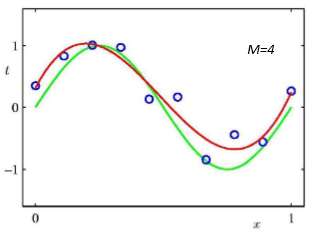
\includegraphics{sections/lec2/3.png}
	\end{center}
	\item For simplicity, we add a \textit{bias function}: $\phi_0 (\vec{x})=1$
	$$\vec{\phi}=1, x, x^2, x^3, \ldots$$
\end{itemize}

\subsection{Basis Function}
\begin{itemize}
	\item Function to construct features from raw data.
	\item e.g.,
	\begin{itemize}
		\item Polynomial: $\phi_j(x)=x^j$
		\item Gaussian: $\phi_j(x)=exp(-\frac{(x-\mu_j)^2}{2s^2})$
		\item Sigmoid: $\phi_j(x)=\sigma (\frac{x-\mu_j}{s})$
	\end{itemize}
\end{itemize}

\subsection{Objective Function}
\begin{itemize}
	\item We will use of sum-of-square errors:
	$$E(w)=\frac{1}{2}\sum_{n=1}^N (y(x^{(n)}, w)-t^{(n)})^2$$
\end{itemize}

\subsection{Batch Gradient Descent}
\begin{itemize}
	\item Given data $(x,y)$ initial $w$, repeat until convergence:
	$$\vec{w}=\vec{w}-\eta \nabla_{\vec{w}} E(\vec{w})$$
	$$\nabla_{\vec{w}}E(w)=\sum_{n=1}^N \left( \sum_{k=0}^{M-1} w_k \phi_k (\vec{x}^{(n)}) - t^{(n)} \right)\phi (\vec{x}^{(n)})=\sum_{n=1}^N \left(\vec{w}^T \phi (\vec{x}^{(n)}) - \vec{t}^{(n)}\right) \phi(x^{(n)})$$
\end{itemize}

\subsection{Overfitting}
\begin{itemize}
	\item An implicit way to tell is when the coeffecients become unreasonably large
	\item Solutions:
	\begin{itemize}
		\item Reduce order
		\item Add more data point
		\item Reselect features, some may be harming you
	\end{itemize}
	\item If you have a small number of data points, then you should use low order polynomial (small number of features)
	\item As you obtain more data points, you can gradually increase the order of the polynomial (more features)
	\item Controlling model complexity: \textbf{regularization}
\end{itemize}

\section{Cameras}
	\subsection{Another kind of factorial}
\begin{lstlisting}[style=C++]
int fact_helper(intn, intresult){
	// REQUIRES: n >= 0
	// EFFECTS: returns result * n!

	if (n == 0) {
		return result;
	}else {
		return fact_helper(n-1,result*n);
	}
}

int factorial(intnum){
	// REQUIRES: num>= 0
	// EFFECTS: returns num!

	return fact_helper(num, 1);
}
\end{lstlisting}

\subsection{Stack effects}
\begin{itemize}
	\item Trace out the stack calls for \lstinline[style=C++]{factorial(2)} for our new and ``old'' function:
	\begin{center}
		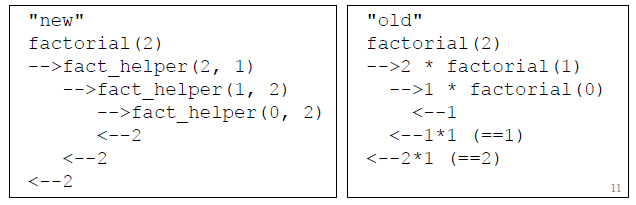
\includegraphics[scale=0.7]{sections/lec3/fact.png}	
	\end{center}

	\item Effects of the new version on the stack:
	\begin{itemize}
		\item The activation record of a function is needed only as long as there is computation left over and can be discarded as soon as the return value is known.
		\item With the new version, the concrete return value isn’t known at the time of the recursive call. However, we do know that whatever that recursive call returns, that will be our return value too.
		\item This means that the caller's stack frame isn't needed any more, and we can throw it away.
	\end{itemize}

	\item This is called \textbf{tail recursion}.
	\item If the result of the recursive call is returned directly with no pending computation, it is tail-recursive. Otherwise, it’s ``plain'' recursion.
\end{itemize}


\section{Camera Calibration}
	\subsection{Tail-recursion to iteration conversion}
\begin{itemize}
	\item There are five steps to the conversion of a tail-recursive function to an iterative one:
	\begin{enumerate}
		\item Copy the function's type signature
		\item Identify any needed ``loop variables'' by inspecting the call to the helper function (if it exists).
		\item Write initialization code to mirror the call to the helper function
		\item Identify termination condition(s) and return values by copying the base case behavior.
		\item Write loop body by copying the inductive step
	\end{enumerate}
\end{itemize}

\subsection{Dependency Graphs}
\begin{itemize}
	\item Special kind of graph with ``directed'' edges showing which ``new'' values depend on which ``old'' values.
	\item An edge is drawn from a \textbf{source vertex} to a \textbf{sink vertex}.
	\item To build a dependency graph, draw one vertex for each variable. If variable fooreads from variable barto compute its new value, draw an edge fromfootobar. (Don't draw an edge between a vertex and itself).
	\item If a variable has no edges with it as a sink(i.e. no edges terminate there), you can write its assignment, and erase it and any edges with it as a source.
	\item If two variables (\lstinline[style=C++]{foo, bar}) are each dependent on the other, then you can solve this by inventing shadow variables:
\begin{lstlisting}[style=C++]
int foo_new = bar - 1; // Shadow variable
int bar_new = foo - 1; // Shadow variable
// ------------------
foo = bar_new;
bar = foo_new;
\end{lstlisting}
	\item The transition between these two steps is called a \textbf{software epoch} - dependencies do not exist across epochs.
\end{itemize}

\section{Single view metrology}
	\subsection{After calibration}
\img{.8}{sections/lec5/p.png}
\begin{itemize}
	\item Internal parameters $K$ are known
	\item $R, T$ are known - but these can only relate $C$ to the calibraiton rig.
	\item You can't estimate $P_i$ from the single image measurement of $p_i$ because it may be anywhere along the line in space.
	\item We also don't have any information in the image to tell us the scale of anything in the world.
\end{itemize}

\subsection{Recovering structure from a single view}
\begin{itemize}
	\item You can make assumptions to get relative sizes of objects in images
	\item Pick a reference plane in the scene
	\item Pick a reference direction (not parallel to the reference plane) in the scene
	\img{.8}{sections/lec5/ref.png}
	\subsubsection{Geometry}
	\img{.8}{sections/lec5/van.png}
	\item Under perspective projection, parallel lines in three-space project to convering lines in the image plane. The common point of intersection, perhaps at infinity, is called the \textbf{vanishing point}
	\begin{itemize}
		\item projection of a point at infinity (goes infinity far)
		\img{.8}{sections/lec5/vp.png}
		\item Any two parallel lines have the same vanishing point
		\item The ray from $C$ through $v$ point is parallel to the lines
		\item AN image may have more than one vanishing point
	\end{itemize}
	\item Two or more vanishing points from lines known to lie in a single 3D plane establish a \textbf{vanishing line}, which completely determines the orientation of the plane
	\img{.7}{sections/lec5/house.png}
\end{itemize}

\subsection{The Cross Ratio}
\img{.8}{sections/lec5/y.png}
\begin{itemize}
	\item $Y$ is desired height to measure
	\item Compute Y from image measurements
	\begin{itemize}
		\item You'll need more than vanishing points to compute this
	\end{itemize}
	\item \textbf{Projective Invariant}: something that does not change under projective transformations (including perspective projection)
	\img{.8}{sections/lec5/l.png}
	\item The \textbf{cross ratio} of 4 collinear points is projective invariant
	$$\frac{||P_3 - P_1||\cdot ||P_4 - P_2||}{||P_3 - P_2||\cdot ||P_4 - P_1||}$$
	\item You can permute the point ordering and it will remain true.
	\item Often called the fundamental invariant of projective geometry
	\img{.8}{sections/lec5/inf.png}
	\item When you consider the points at $\infty$, and the point where the camera would meet the ground plane $v_z$ you have enough points to use the cross ratio on our camera model.
	\item You need the same points in the world and camera system (can't mix and match)
	\item You must make some assumption to determine the relative sizes, typically assume $L$
\end{itemize}

\subsection{Horizon line}
\img{.7}{sections/lec5/hor.png}
\begin{itemize}
	\item Sets of parallel lines on the same plane lead to collinear vanishing points the line is called the \textbf{horizon}
	\img{.8}{sections/lec5/ex.png}
	\item When trying to recover the structure within the camera reference system, we can check if two linesare parallel or not
	\begin{itemize}
		\item If they do, recognize the horizon line
		\item Measure if hte 2 lines meet the horizon
		\item If they do, they are parallel in 3D
		\item Actual scale of scene is not recovered, only relative distances
	\end{itemize}
\end{itemize}

\subsection{Lines in a 2D plane}
$$ax+by+c=0; l=\begin{bmatrix}
	a\\b\\c
\end{bmatrix}$$
\subsubsection{Intersecting lines}
\img{1}{sections/lec5/intersect.png}
\begin{itemize}
	\item The intersection of lines can be calculated with: 
	$$x=l\times l'$$
\end{itemize}

\subsection{Stereo-view geometry}
\img{1}{sections/lec5/tri.png}
\begin{itemize}
	\item Two camera perspectives allow us to find position of objects through \textbf{triangulation}
	\begin{itemize}
		\item This requires a few knowns, $K_1, K_2, R, T$
	\end{itemize}
	\item Small inaccuracies with knowns can lead to situations where the lines may not intersect 
	\item Instead, we'll find where they came close enough
		$$d^2(x_1, M_1X)+d^2(x_2, M_2X)$$
		$$d:=\text{distance between two lines}$$
\end{itemize}

\subsection{Epipolar Geometry}
\img{.7}{sections/lec5/ep.png}
\begin{itemize}
	\item \textbf{Epipolar plane} (grey): intersections of baseline with image planes
	\item \textbf{Baseline} (orange): projectison of other camera center
	\item \textbf{Epipolar lines} (blue): vanishing points of camera motion direction
	\item This framepoint, allows us to consider if two pointsare related by epipolar geometry
	\item Use epipolar lines to find sharing points will greatly save computation cost as a 2D search becomes 1D
	\subsubsection{Parallel image planes}
	\item Baseline intersects the image plane at infinity
	\item Epipoles are at infinity
	\item Epipolar lines are parallel to x-axis
	\subsubsection{Forward translation}
	\img{1}{sections/lec5/f.png}
	\item When a camera moves forward the lines turn into a spiral
\end{itemize}

\end{document}